\documentclass[pdftex,12pt]{article}

\usepackage{fancyvrb}				% for Verbatim environments
\usepackage{color}

%\usepackage[a4paper]{geometry}		%	Flexible and complete interface to document dimensions (scalebox,...)
\usepackage[top=2cm,footskip=2cm]{geometry}

\usepackage{pxfonts}				%	Palatino-like fonts in support of mathematics
\usepackage{adjustbox}				%	for \textwidth and a lot more
\usepackage{multicol}				%	multipe columns
\usepackage{wasysym}
\usepackage{varwidth}
\usepackage{tikz}
\usepackage{listings}

\usepackage{tcolorbox}
\tcbuselibrary{breakable}

\usepackage{imakeidx}
\makeindex[intoc]
\renewcommand{\indexname}{Index of keywords}

%	Use adjustwidth environment to exceed column width (see example table in text)
\usepackage{changepage}

%	Extensive support for hypertext in LaTeX (linking ToC to text)
\usepackage[pdftex,citecolor=black,linkcolor=blue,urlcolor=blue,colorlinks]{hyperref}

% code block
\newenvironment{codebox}
{\begin{tcolorbox}[colback=blue!10!gray!10, colframe=blue!10!gray!40, boxrule=0.5pt, breakable]}
{\end{tcolorbox}}

% note block
\newenvironment{notebox}
{\begin{tcolorbox}[colback=white,colframe=red!55!black,boxrule=1pt, left skip=2cm, right skip=2cm, title=\textbf{Note}]}
{\end{tcolorbox}}

% inline code block : http://tex.stackexchange.com/questions/203848/problem-with-underscores-in-newcommand
\newcommand{\incode}[1]{\tcbox[colback=blue!10!gray!10, colframe=blue!10!gray!40, boxrule=0.5pt, on line, size=fbox]{\texttt{\detokenize{#1}}}}
% inline code block : a variant for environments such as section headers, math & more...
\newcommand{\incodeEnv}[1]{\tcbox[colback=blue!10!gray!10, colframe=blue!10!gray!40, boxrule=0.5pt, on line, size=fbox]{\texttt{#1}}}

% verbatim styled index but underscore characters still need to be escaped!
\newcommand{\Index}[1]{\index{#1@\texttt{#1}}}
\newcommand{\IndexSub}[2]{\index{#1@\texttt{#1}!#2@\texttt{#2}}}

% styled pageref
\newcommand{\pref}[1]{see  Pg.~\pageref{#1}}

% ABLE keyword
\newcommand{\ABLE}{\incode{ABLE}}

% small hyperref T1, T2, T3
\newcommand{\TOne}{{\footnotesize (\hyperref[T1_T2_T3]{T1})}}		%	small T1
\newcommand{\TTwo}{{\footnotesize (\hyperref[T1_T2_T3]{T2})}}		%	small T2
\newcommand{\TThree}{{\footnotesize (\hyperref[T1_T2_T3]{T3})}}		%	small T3

% red coloured text
\newcommand{\RED}[1]{\textcolor{red}{\detokenize{#1}}}



\begin{document}

%opening
\begin{titlepage}
\centering
\vspace*{\fill}

\begin{center}
\begin{adjustwidth}{2.4in}{0in}
	\begin{itemize}
		\item [{\Huge \textbf{A}}] pproximate
		\item [{\Huge \textbf{B}}] lockwise
		\item [{\Huge \textbf{L}}] ikelihood
		\item [{\Huge \textbf{E}}] stimation
	\end{itemize}
\end{adjustwidth}
\end{center}

\vspace{1cm}

Version 0.1.1 \\
\today

\vspace{2cm}

{\large Champak Beeravolu Reddy}

\href{mailto:champak.br@gmail.com}{champak.br@gmail.com}

\vspace*{\fill}
\end{titlepage}

\vspace*{3cm}
\tableofcontents
\vspace*{\fill}

\clearpage


\section{Introduction}
\ABLE\ is a program written in C/C++ for the joint inference of arbitrary population histories and the genome-wide recombination rate using data from multiple whole genome sequences or fragmented assemblies (e.g. UCE's, RADSeq, and targeted exomes). The inference results in a Maximum Likelihood Estimate (MLE) of the parameters corresponding to the demographic model of interest along with the recombination parameter. It makes use of the distribution of blockwise SFS (bSFS) patterns which retain information on the variation in genealogies or Ancestral Recombination Graphs (ARGs) spanning short-range linkage blocks across the genome. \ABLE\ does not require phased data as the bSFS does not distinguish the sampled lineage in which a mutation has occurred. Like with the SFS, outgroup information can be also be ignored by folding the bSFS. \ABLE\ takes advantage of \incode{openmp} parallelization and is tailored for studying the population histories of model as well as non-model species.

This is the documentation accompanying \ABLE\ and the current version of the project is freely available from \url{https://github.com/champost/ABLE}. 


\section{Installation}
\subsection{Linux}
It is easiest to build an \incode{ABLE} binary under all flavours of Linux. \incode{ABLE} requires the GNU Compiler Collection (\incodeEnv{\href{https://gcc.gnu.org/}{gcc}}) 
and GNU Make (\incodeEnv{\href{https://www.gnu.org/software/make/}{make}})
for a smooth installation and has been tested using \incode{gcc 4.8.4} and \incode{make 3.81}. It is also useful to have \incodeEnv{\href{https://git-scm.com/}{git}} installed for seamless updates of the latest version of \incode{ABLE}. If you do not have \incode{gcc}, \incode{make} or \incode{git}, you can use your OS specific package handling utility. 

Under Ubuntu this corresponds to the following in a terminal

	\begin{codebox}
		\begin{verbatim}
sudo apt-get install build-essential git
		\end{verbatim}
	\end{codebox}
Other dependencies such as the GNU Scientific Library (\incodeEnv{\href{http://www.gnu.org/software/gsl/}{GSL}}) and the Non-Linear Optimization (\incodeEnv{\href{http://ab-initio.mit.edu/wiki/index.php/NLopt}{NLopt}}) library are automatically installed by following the instructions outlined below.

\begin{enumerate}
%1. Clone the `ABLE` repository. If `git` is not available see the next section (or [here](https://git-scm.com/downloads)).
%
%git clone https://github.com/champost/ABLE.git
%
%2. Change directory
%
%cd ABLE
%
%3. If you are installing `ABLE` for the **first time** you might have to compile the `GSL` and `NLopt` libraries from source. This can take some time as the command below performs a **static installation** of the libraries. You can skip this step if you already have these libraries installed system-wide or if you are simply updating `ABLE` to the latest version (see next section).
%
%make deps
%
%4. Finally, build an `ABLE` binary
%
%make clean && make all
	
	
	
	\item Clone the \incode{ABLE} repository. If \incode{git} is not available see the next section (or \href{https://git-scm.com/downloads}{here}).
	
	\begin{codebox}
		\begin{verbatim}
		git clone https://github.com/champost/ABLE.git
		\end{verbatim}
	\end{codebox}
	
	\item Change directory
	
	\begin{codebox}
		\begin{verbatim}
		cd ABLE
		\end{verbatim}
	\end{codebox}
	
	\item If you are installing \incode{ABLE} for the \underline{\textbf{first time}} you might have to compile the \textbf{GSL} and \textbf{NLopt} from source. This can take some time as the command below performs a \textbf{static installation} of the libraries. You can skip this step if you already have these libraries installed system-wide or if you are simply updating \ABLE\ to the latest version (see next section).
	
	\begin{codebox}
		\begin{verbatim}
		make deps
		\end{verbatim}
	\end{codebox}
	
	\item Finally, build an \incode{ABLE} binary
	
	\begin{codebox}
		\begin{verbatim}
		make clean && make all
		\end{verbatim}
	\end{codebox}
\end{enumerate}
If you want \incode{ABLE} to be accessible from everywhere, such as your data folder, you might want to

	\begin{codebox}
		\texttt{cp ABLE $ \sim $/bin}
	\end{codebox}

This ensures that you can execute the program by specifying \incode{ABLE ...} instead of \incode{./ABLE ...} from the installation folder. This holds only if \incodeEnv{$ \sim $/bin} exists and is part of your \incodeEnv{\$PATH} environment variable.


\section{Updates}
\subsection{With Git}
As mentioned above, \incode{git} considerably simplifies the process (or headache) of updating \incode{ABLE}. You simply have to change your current working directory to that of \incode{ABLE} and execute the following

\begin{codebox}
	\begin{verbatim}
	git pull
	make clean && make all
	\end{verbatim}
\end{codebox}


\subsection{Without Git}
If \incode{git} is not available on your machine you can try looking for solutions \href{https://git-scm.com/downloads}{here}. Alternatively, you can download the \incode{ABLE} repository somewhere on your computer as shown below.

\begin{codebox}
	\begin{verbatim}
	wget https://github.com/champost/ABLE/archive/master.tar.gz
	\end{verbatim}
\end{codebox}

Untar the archive using
\begin{codebox}
	\begin{verbatim}
	tar -xzf master.tar.gz
	\end{verbatim}
\end{codebox}
and manually compare the contents of the \incode{ABLE-master} directory with your \incode{ABLE} installation and replace the files that have changed in size.
	
\subsection{Updating dependencies}
With or without \incode{git}, you will seldom need to recompile the libraries that \incode{ABLE} depends upon and in which case you will have to run the \incode{make deps} command before compiling an \incode{ABLE} binary with \incode{make clean && make all}. This information will be clearly stated in the \href{https://github.com/champost/ABLE/releases}{Release notes} and/or the \incode{ABLE} \href{https://github.com/champost/ABLE/blob/master/doc/helpABLE.pdf}{documentation}.



\section{Configuration}
For \ABLE\ to execute correctly, you need to specify a command line, some options in a config file and provide a data file.


\subsection{Command line options} 
\label{cmdline} 
The command line needs to be in the \textbf{\textit{ms}} format. Note that \ABLE\ supports only a subset (shown below) of all the available \textbf{\textit{ms}} command line options. Please refer to the \href{http://home.uchicago.edu/rhudson1/source/mksamples.html}{full \textbf{\textit{ms}} documentation} for a better understanding of these options.
\begin{tcolorbox}[colback=white,colframe=black,boxrule=1pt]
	\begin{multicols}{2}
		\begin{itemize}
			\item \verb|-t| $ \theta $
			\item \verb|-r| $ \rho $ \textbf{nsites}
			\item \verb|-G| $ \alpha $
			\item \verb|-I| npop n1 n2 ... $ [4N_{0}m] $
			\item \verb|-eG| $ t\ \alpha $
			\item \verb|-eg| $ t\ i\ \alpha_{i} $
			\item \verb|-eN| $ t\ x $
			\item \verb|-en| $ t\ i\ x $
			\item \verb|-eM| $ t\ x $
			\item \verb|-em| $ t\ i\ j\ x $
			\item \verb|-ema| $ t $ npop $ M_{11}\ M_{12}\ M_{13}...\ M_{21}\ ... $
			\item \verb|-es| $ t\ i\ p $
			\item \verb|-ej| $ t\ i\ j $
		\end{itemize}
	\end{multicols}
\end{tcolorbox}


\subsubsection{The \incode{tbi} keyword} 
\label{key:tbi} 
\Index{tbi}
While {\textbf{\textit{ms}}} provides for the \incode{tbs} option, we introduce the \incode{tbi} keyword which stands for "\textbf{to be inferred}" as part of the \ABLE\ command line. \incode{tbi} keywords are to be used instead of the values of the parameters of a demographic model (\textit{i.e.} some floating value) which need to be inferred. All \incode{tbi} keywords need to be suffixed by a number (\incode{tbi1, tbi2,...}). Thus, all occurrences on the command line of the same demographic parameter can be correctly identified. 

Below is a typical example of an \ABLE\ command line for a simple history describing a single discrete change in population size defined by three parameters (current and ancestral population sizes and the time of size change) which are to be inferred (see \ref{sec:examples_exact_bSFS}):
	\begin{codebox}
		\begin{verbatim}
./ABLE 4 100000 -t tbi1 -eN tbi2 tbi3 -T config.txt
		\end{verbatim}
	\end{codebox}

\ABLE\ also requires the user to specify a \incode{-T} towards the end of the command line indicating the start of the config filename (if any) specified by the user. If no filename is specified, by default \ABLE\ looks for a file called \incode{config.txt}.


\subsection{Config file options} 
\label{configfile}
\begin{notebox}
	\begin{itemize}
		\item \textbf{All options} of the config file are \textbf{case sensitive}.
		\item Successive options can undo previous ones.
	\end{itemize}
\end{notebox}


\subsubsection{Syntax}
\Index{\#~(commented line)}
Any line in the config file beginning with the hash symbol \incodeEnv{\#} will be considered as a comment by \ABLE\ and ignored. Every keyword along with its corresponding options are to be specified on a separate line. Also, keywords and options are to be separated by a single space. All config file keywords introduced here will be of one or more of these types :

\begin{itemize}
\item [\textcolor{blue}{T1} : ] \incode{Key} 
\item [\textcolor{blue}{T2} : ] \incode{Key val} \textit{or} \incode{Key val1 val2 val3 ...}
\item [\textcolor{blue}{T3} : ] \incode{Key SubKey val} \textit{or} \incode{Key SubKey val1 val2 val3...}
\phantomsection
\label{T1_T2_T3}
\end{itemize}
Here, the presence/absence of a \textcolor{blue}{T1} keyword respectively represents a binary true/false option whereas it is possible to specify a lot more with a \textcolor{blue}{T2}/\textcolor{blue}{T3} keyword. 


\subsubsection{Keywords}

 	\begin{notebox}
 		Comments need to be specified as an entire line in \ABLE . \textbf{Unexpected behaviour} can result if you specify keywords/options and a comment on the \textbf{same line} \textit{e.g.} \incodeEnv{Key val \# \textit{comment after keyword}}
 	\end{notebox}

\begin{itemize}
	\item[\RIGHTarrow] \incode{datafile} \TTwo \\
	\Index{datafile}
	Accepts a single value specifying the name and location (relative to the config file) of the file containing the data (see \ref{sec:data_format} for more on the data format).
	
	\begin{codebox}
		\begin{verbatim}
		datafile filename
		\end{verbatim}
	\end{codebox}
	
	\item[\RIGHTarrow] \incode{datafile_format} \TTwo \\
 	\Index{datafile\_format}
	\phantomsection
	\label{key:data_format}
 	Data can be specified in either of the two formats below. 
 	
 	\begin{notebox}
 		The \textbf{default} input file format is \incode{bSFS}.
 	\end{notebox}

	\begin{itemize}
	 	\item \incode{datafile_format bSFS} \\
	 	\IndexSub{datafile\_format}{bSFS}
	 	Each line in this format contains a tag describing the bSFS configuration (joint bSFS if multiple population samples) and its respective frequency of occurrence in the data. 
		\begin{codebox}
			\begin{verbatim}
			(tag1) : prob1
			(tag2) : prob2
			...
			\end{verbatim}
		\end{codebox}
		For an example of this format please refer to the accompanying Orangutan dataset in the \incode{/data} folder. Further information on the general logic behind the bSFS/jbSFS tags will be provided here later.

	 	\item \incode{datafile_format pseudo_MS} \\
	 	\IndexSub{datafile\_format}{pseudo\_MS}
	 	This format closely resembles that of simulated samples output by the \href{http://home.uchicago.edu/rhudson1/source/mksamples.html}{\textbf{\textit{ms}}} software and will be the easiest for all users of \ABLE\ to provide. A more detailed description of this format can be found in \ref{sec:data_format}. A file named \incode{block_SNPs.txt} is created with the number of SNPs per sequence block providing for a manual cross-check that \ABLE\ has correctly accounted for available polymorphism. While tri/quadri-allelic nucleotide positions are ignored they are however listed in \incode{block_SNPs.txt}.
	\end{itemize}
	
	\item[\RIGHTarrow] \incode{allele_type} \TTwo \\
 	\Index{allele\_type}
	\phantomsection
	\label{key:allele_type}
	This option provides additional information to \ABLE\ on how to read in the data when it is already in a \incode{pseudo_MS} format. See \ref{sec:data_format} for full examples of both the formats below.
	
	\begin{itemize}
	 	\item \incode{allele_type genotype} \\
	 	\IndexSub{allele\_type}{genotype}
		Valid characters are \incode{A}, \incode{T}, \incode{G} or \incode{C} and missing information is specified by using \incode{N} (see \ref{sec:data_genotype}).
		
	 	\item \incode{allele_type binary} \\
	 	\IndexSub{allele\_type}{binary}
		Valid characters are \incode{0} or \incode{1} and missing information is specified by using \incode{N}  (see \ref{sec:data_binary}).
	\end{itemize}
	
	\item[\RIGHTarrow] \incode{task} \TTwo\ \\
 	\Index{task}
	\phantomsection
 	\label{key:task}
	This option defines any one of the three principal tasks (or modes) that \ABLE\ is meant to undertake. More information can be found in the examples section (\ref{sec:examples}).
	\begin{itemize}
	 	\item \incode{task exact_bSFS} \\
		\IndexSub{task}{exact\_bSFS}
	 	\ABLE\ attempts to calculate the \textbf{exact bSFS} for a given number of genealogies to be sampled and there is no requirement for a file containing data. Results obtained under this mode can be readily compared with analytical results. A file named \incode{expected_bSFS.txt} is generated with the expected bSFS for a given number of genealogies and a point in parameter space (see \ref{sec:examples_exact_bSFS}).

	 	\item \incode{task conditional_bSFS} \\
		\IndexSub{task}{conditional\_bSFS}
	 	This mode of \ABLE\ calculates the \textbf{conditional bSFS} (\textit{i.e.} only configurations found in the data) at a given point in parameter space and for some number of genealogies (see \ref{sec:examples_conditional_bSFS}). 

	 	\item \incode{task infer} \\
	 	\IndexSub{task}{infer}
	 	This is the standard mode for inferring demographic parameters and will be the most used feature of \ABLE. This mode typically consists of a global search followed by a local search and finally a refined log-likelihood (\textit{lnL}) at the MLE (see \ref{sec:examples_inference}).
	\end{itemize}
	
	
 	\begin{notebox}
 		\ABLE\ expects \incode{tbi} keywords as part of the \incode{ms} command-line \textbf{only for} the \incode{task infer} mode. (See also \incode{profile_likelihoods} on pg.~\pageref{key:profile_likelihoods}). 
	\end{notebox}
	
	\item[\RIGHTarrow] \incode{bSFS} \TTwo \\
	\Index{bSFS}
	Accepts a single value specifying the name and location (relative to the config file) of the bSFS output file for the \incode{exact_bSFS} and \incode{conditional_bSFS} cases (see above). The bSFS output is thus for a given demographic model, at a point in parameter space and for a specified number of genealogies.
	\begin{codebox}
		\begin{verbatim}
		bSFS filename
		\end{verbatim}
	\end{codebox} 
	The default name of the output file is \incode{bSFS.txt}.
	
	\item[\RIGHTarrow] \incode{kmax} \TTwo \\
	\Index{kmax}
	\phantomsection
	\label{key:kmax}
	A single argument following this keyword specifies the maximum number of mutation classes at single nucleotide sites (\textit{i.e.} singletons, doubletons, \textit{etc.}) to be explicitly accounted for in the bSFS. Mutations appearing more frequently in your data than the specified \incode{kmax} are not ignored but rather grouped into a marginal probability class. A maximum of 3 is specified as follows
	\begin{codebox}
		\begin{verbatim}
		kmax 3
		\end{verbatim}
	\end{codebox} 
	Thus, when sampling genealogies/ARGs, \ABLE\ will account for 0, 1, 2 and 3 SNPs in all blocks and bundle the probability of observing more the 3 SNPs into a marginal probability.
	
	\item[\RIGHTarrow] \incode{folded} \TOne \\
	\Index{folded}
	The presence of this keyword instructs \ABLE\ to consider the "polarity" \textit{i.e.} account for the ancestral/derived states of alleles with respect to an outgroup and thus use the folded bSFS. If the data is not in a binary format (\pref{sec:data_genotype}) then the first allele at every nucleotide position in the first population is taken to be of the ancestral type.
	
	\item[\RIGHTarrow] \incode{pops} \TThree \\
	\Index{pops}
	\phantomsection
	\label{key:pops}
	This option takes as a first argument the number of population samples that will be analysed followed by the number of samples per population in the order that they have been specified on the \textbf{\textit{ms}} command line
	\begin{codebox}
		\begin{verbatim}
		pops npops n1 n2 n3 ...
		\end{verbatim}
	\end{codebox} 
	For a single population example with 5 genomes it should be
	\begin{codebox}
		\begin{verbatim}
		pops 1 5
		\end{verbatim}
	\end{codebox} 
	whereas for a 3 population example with 1, 4 and 2 genomes respectively it should be specified as
	\begin{codebox}
		\begin{verbatim}
		pops 3 1 4 2
		\end{verbatim}
	\end{codebox} 
	
	\item[\RIGHTarrow] \incode{convert_data_to_bSFS} \TTwo \\
	\Index{convert\_data\_to\_bSFS}
	With this option \ABLE\ simply converts a \incode{pseudo_MS} format file into the bSFS format. It is advised for users to store data in the bSFS format (especially for large samples) as it is quicker to load and because internally \ABLE\ works with the bSFS. When asked to convert data, \ABLE\ performs the task, creates a \incode{block_SNPs.txt} file like in the case of \incode{datafile_format pseudo_MS} (\pref{key:data_format}) and terminates. For the conversion you can run \incode{./ABLE config.txt} in the terminal with the contents of \incode{config.txt} as below
	\begin{codebox}
		\begin{verbatim}
		# (modify the "pops" option according to your sampling)
		pops 2 4 4
		datafile input_filename
		convert_data_to_bSFS output_filename
		\end{verbatim}
	\end{codebox}
	
	\item[\RIGHTarrow] \incode{start} \TTwo/\TThree \\
 	\Index{start}
	\phantomsection
	\label{key:start}
	This applies only when \incode{tbi} keywords have been specified as part of the command line (see \ref{cmdline}) and need to be initialized with numeric values from within the config file.
	\begin{itemize}
		\item \incode{start all val1 val2 ...} \\
		\IndexSub{start}{all}
		When all parameters need to be initialized at once with respect to the "\incode{tbi} order". Let us assume that your demographic model contains three free parameters, \incode{tbi2}, \incode{tbi3} and \incode{tbi7}. If you want to initialize these parameters with \incode{tbi7 = 10}, \incode{tbi2 = 5.2} and \incode{tbi3 = 1}, then
		\begin{codebox}
			\begin{verbatim}
			start all 5.2 1 10
			\end{verbatim}
		\end{codebox} 
		
		\item \incode{start random} \\
		\IndexSub{start}{random}
		Initializes all \incode{tbi} keywords with uniformly drawn random values over the respective bounds of each demographic parameter. 	The default lower and upper bounds for all parameters are $ 10^{-3} $ and 5 respectively.
		
		
		\item \incode{start tbi val} \\
		\IndexSub{start}{tbi}
		If a single \incode{tbi} parameter needs to be initialized (\textit{e.g.} \incode{tbi4 = 3}), then
		\begin{codebox}
			\begin{verbatim}
			start tbi4 3
			\end{verbatim}
		\end{codebox} 
	\end{itemize}
	
	\item[\RIGHTarrow] \incode{profile} \TThree \\
	\Index{profile}
	\IndexSub{profile}{tbi}
	\phantomsection
	\label{key:profile}
	This applies only when the \incode{profile_likelihoods} keyword has been specified (\pref{key:profile_likelihoods}) in the config file and \incode{tbi} keywords as part of the command line (see \ref{cmdline}). It enables the user to explore a grid in \textit{n} dimensions (i.e. number of \incode{tbi} params) for which \ABLE\ outputs a list of likelihoods making it easy to plot the discretized profile likelihood. For each parameter the discrete exploration of likelihoods can be specified as follows \incode{profile tbi val1 val2 ...}
	
	Below is an example for four \incode{tbi} parameters which tells \ABLE\ to explore all combinations starting with \incode{(0.1,0.1,0.6,0.1)} to \incode{(0.5,0.3,0.7,0.3)}.
	\begin{codebox}
	\begin{verbatim}
		profile_likelihoods 500
		
		profile tbi2 0.1 0.3 0.5
		profile tbi4 0.1 0.2 0.3
		profile tbi5 0.6 0.7
		profile tbi7 0.1 0.2 0.3
	\end{verbatim}
	\end{codebox}
	Note that unexpected behaviour may result if the \incode{start} keyword (\pref{key:start}) is used in conjunction with this option.

	\item[\RIGHTarrow] \incode{global_search} \TTwo \\
 	\Index{global\_search}
	This option sets the global search strategy for the MLE and makes use of the algorithms implemented in the \href{http://ab-initio.mit.edu/wiki/index.php/NLopt}{NLopt library}.
	\begin{itemize}
		\item \incode{global_search DIRECT} \\
		\IndexSub{global\_search}{DIRECT}
		Uses the DIviding RECTangles  (\href{http://ab-initio.mit.edu/wiki/index.php/NLopt_Algorithms#DIRECT_and_DIRECT-L}{DIRECT}) algorithm for global optimization.

		\item \incode{global_search CRS} \\
		\IndexSub{global\_search}{CRS}
		Uses the Controlled Random Search with local mutation (\href{http://ab-initio.mit.edu/wiki/index.php/NLopt_Algorithms#Controlled_Random_Search_.28CRS.29_with_local_mutation}{CRS}) algorithm for global optimization.

		\item \incode{global_search ISRES} \\
		\IndexSub{global\_search}{ISRES}
		Uses the Improved Stochastic Ranking Evolution Strategy (\href{http://ab-initio.mit.edu/wiki/index.php/NLopt_Algorithms#ISRES_.28Improved_Stochastic_Ranking_Evolution_Strategy.29}{ISRES}) algorithm for global optimization.

		\item \incode{global_search ESCH} \\
		\IndexSub{global\_search}{ESCH}
		Uses the Evolutionary Strategies algorithm by Carlos Henrique da Silva Santos (\href{http://ab-initio.mit.edu/wiki/index.php/NLopt_Algorithms#ESCH_.28evolutionary_algorithm.29}{ESCH}) for global optimization.
	\end{itemize}
	
	\item[\RIGHTarrow] \incode{global_search_trees} \TTwo \\
	\Index{global\_search\_trees}
	Accepts a single value which specifies the number of genealogies/ARGs to be sampled during the \textbf{global search} of the MLE. The default number of genealogies is 10,000. This corresponds to the precision of the likelihood to be used during this search.
	
	\item[\RIGHTarrow] \incode{local_search_trees} \TTwo \\
	\Index{local\_search\_trees}
	Accepts a single value which specifies the number of genealogies/ARGs to be sampled during the \textbf{local search} of the MLE. The default number of genealogies is 15,000. This corresponds to the precision of the likelihood to be used during this search.
	
	\item[\RIGHTarrow] \incode{global_search_evals} \TTwo \\
	\Index{global\_search\_evals}
	Accepts a single value which specifies the number of points in parameter space that should be explored before concluding the \textbf{global search} for the MLE. The default number of evaluations is \textbf{2,000} times the number of \incode{tbi} parameters. A warning is issued if the user specifies a number below the default value.
	
	\item[\RIGHTarrow] \incode{local_search_evals} \TTwo \\
	\Index{local\_search\_evals}
	Accepts a single value which specifies the number of points in parameter space that should be explored before concluding the \textbf{local search} for the MLE. The default number of evaluations is \textbf{1,000} times the number of \incode{tbi} parameters. A warning is issued if the user specifies a number below the default value.
		
	\item[\RIGHTarrow] \incode{global_upper_bound} \TTwo \\
	\Index{global\_upper\_bound}
	Accepts a single value which defines the \textbf{upper bound} for all \incode{tbi} parameters though this can be undone for certain by specifying individual bounds (see the \incode{bounds} keyword). The default upper bound for all parameters is~5.
	
	\item[\RIGHTarrow] \incode{global_lower_bound} \TTwo \\
	\Index{global\_lower\_bound}
	Accepts a single value which defines the \textbf{lower bound} for all \incode{tbi} parameters though this can be undone for certain by specifying individual bounds (see the \incode{bounds} keyword). The default lower bound for all parameters is~$ 10^{-3} $.
	
	\item[\RIGHTarrow] \incode{skip_global_search} \TOne \\
	\Index{skip\_global\_search}
	This keyword skips the global search and starts the local search directly with the user-specified start point in parameter space with the help of the \incode{start} keyword (\pref{key:start}).
	
	\item[\RIGHTarrow] \incode{skip_local_search} \TOne \\
	\Index{skip\_local\_search}
	This keyword modifies the default behaviour of \incode{ABLE} and skips the local search after the global search.
	
	\item[\RIGHTarrow] \incode{bounds} \TThree \\
	\Index{bounds}
	Individual parameter bounds during the MLE search can be set with this keyword. The \incode{tbi} parameter needs to be specified as the second keyword and followed by the minimum and maximum bounds respectively. So if you want to impose \incode{0.5 < tbi2 < 4.2}, then
	\begin{codebox}
		\begin{verbatim}
		bounds tbi2 0.5 4.2
		\end{verbatim}
	\end{codebox} 
	The default lower and upper bounds for all parameters are $ 10^{-3} $ and 5 respectively.
	
	\item[\RIGHTarrow] \incode{constrain} \TTwo \\
	\Index{constrain}
	Presently in \ABLE, it is possible to specify simple parameter constraints to enforce biological coherence between two demographic events \textit{e.g.} gene flow is necessarily a more recent event than divergence in a two population model. Multiple constraints can be specified (each on a separate line) and each constraint only accepts two \incode{tbi} parameters. For example, in order to impose the constraint \incode{tbi4 < tbi2}, specify
	\begin{codebox}
		\begin{verbatim}
		constrain tbi4 tbi2
		\end{verbatim}
	\end{codebox} 
	and in this very order.
	
	%	\item \incode{no_profiles} \TOne \\
	%	Code in development...to be written.
	
	%	\item \incode{only_profiles} \TOne \\
	%	Code in development...to be written.
	
	\item[\RIGHTarrow] \incode{seed_PRNG} \TTwo \\
	\Index{seed\_PRNG}
	Accepts a single value which acts as the starting seed for the Pseudo random Number Generator (PRNG) which follows the Mersenne Twister algortihm (as implemented in the \href{http://www.gnu.org/software/gsl/}{GNU Scientific Library}). By default, \ABLE\ uses all available threads on a system for computation (see also \incode{set_threads} option), and automatically attributes a different seed to each thread by successively incrementing the user-specified start value by 1. If no value was specified, \ABLE\ uses the state of the system clock to generate a seed and then attributes a seed by successive incrementation to each thread.
		
	\item[\RIGHTarrow] \incode{refine_likelihoods} \TTwo \\
	\Index{refine\_likelihoods}
	Accepts a single value which specifies the number of genealogies to be sampled for a further refinement of the Monte Carlo \textit{lnL} at the MLE found after a global/local search.
	
	\item[\RIGHTarrow] \incode{profile_likelihoods} \TTwo \\
	\Index{profile\_likelihoods}
	\phantomsection
	\label{key:profile_likelihoods}
	Accepts a single value which specifies the number of genealogies to be sampled for calculating the Monte Carlo \textit{lnL} at the user-specified discrete parameter combinations. This is equivalent to specifying \incode{task conditional_bSFS} (\pref{key:task}) but differs in that it needs \incode{tbi} keywords and makes use of the \incode{profile} keyword (\pref{key:profile}) for specifying the grid.

	\item[\RIGHTarrow] \incode{report_likelihoods} \TTwo \\
	\Index{report\_likelihoods}
	Accepts a single value which asks \ABLE\ to report the parameter point with the best MLE during the (global or local) search after the specified number of likelihood evaluations.
	
	\item[\RIGHTarrow] \incode{start_likelihood} \TTwo \\
	\Index{start\_likelihood}
	Accepts a single value which is a user-specified \textit{lnL} and \ABLE\ is asked to check if it can improve over this value during a local search. This option applies only when the \incode{skip_global_search} keyword has been specified.
	
	\item[\RIGHTarrow] \incode{no_bSFS_file} \TOne \\
	\Index{no\_bSFS\_file}
	This asks \ABLE\ not to output a bSFS file. Only standard information such as the \textit{lnL} and computation time are written to the console.
	
	\item[\RIGHTarrow] \incode{print_correction_factor} \TOne \\
	\Index{print\_correction\_factor}
	This option asks \ABLE\ to print the correction factor ($ \geq 1 $) which penalizes the likelihood at a point in parameter space. These situations can arise when the number of genealogies specified by the user are insufficient for explaining all the bSFS configurations present in the data. Or when you are attempting to fit the data without recombination when the data bSFS contains configurations which violate the four gamete test. The printing is only activate when \incode{task conditional_bSFS} (\pref{key:task}) and a value greater than 1 indicates that the penalization is in effect.
	
	\item[\RIGHTarrow] \incode{set_ftol_abs} \TTwo \\
	\Index{set\_ftol\_abs}
	Accepts a single value which sets the tolerance in terms of the difference in absolute value between successive evaluations at points in parameter space during the local search. Let $ \epsilon $ be the user provided value and assume that the local search has evaluated the likelihood function, $ f(x) $, at points $ x_{1} $ and then $ x_{2} $. If the condition $ |f(x_{2}) - f(x_{2})| < \epsilon $ is satisfied, the search is terminated and the MLE is reported by \ABLE.
	
	\item[\RIGHTarrow] \incode{set_threads} \TTwo \\
	\Index{set\_threads}
	Accepts a single value indicating the number of threads that \ABLE\ needs to spawn for a parallel computation of the bSFS likelihoods.
	
\end{itemize}


\subsection{Data format} 
\label{sec:data_format}
\ABLE\ accepts data in simple text files which can be in either of two formats : \incode{pseudo_MS} or \incode{bSFS} (\pref{key:data_format}). If you have your data in other formats (\textit{e.g.} VCF,...), then converting it into the \incode{pseudo_MS} should be very easy. The order in which population samples need to be input closely resembles the \href{http://home.uchicago.edu/rhudson1/source/mksamples.html}{\textbf{\textit{ms}}} format. Briefly, the samples from each population for which you will have attributed an \textit{a priori} order (\incode{pops} keyword, \pref{key:pops}) should be listed.

By default, the \incode{pseudo_MS} format expects sequence blocks using only the genotype information (\textit{i.e.} \incode{A/T/G/C/N}). If you have prior information regarding the ancestral/derived states at each segregating site you can specify the blocks in a binary format (using the \incode{allele_type} option, \pref{key:allele_type}), in which case all sequences must be in this format. Nucleotide positions containing a \incode{N} (\textit{e.g.} due to missing information) will be completely ignored as are tri/quadri-allelic SNPs.


\subsubsection{The \incodeEnv{pseudo\_MS} genotype format}
\IndexSub{datafile\_format}{pseudo\_MS}
\IndexSub{allele\_type}{genotype}
\label{sec:data_genotype}
Each block begins with a \incode{//} followed by an optional header which can span any number of lines. Below is an example of three sequence blocks -- a Chr7 block, a fictional monomorphic block and from Chr4 respectively -- from the accompanying 2kb Orangutan dataset (\incode{/data} folder). The first four samples (2 diploids) are from the Bornean population and the rest are from Sumatran individuals. The corresponding population order is \incode{pops 2 4 4} (\pref{key:pops}).


\begin{notebox}
	Headers \textbf{may not begin} with either of \incode{A}, \incode{T}, \incode{G}, \incode{C} or \incode{N} characters! Use a \incodeEnv{\#} to start a line if necessary.
\end{notebox}

\begin{codebox}
	\begin{verbatim}
	//
	7_41030400-41032000
	TCATCTG
	TCATCTG
	GCATTGT
	GCATTGT
	GCAGCGG
	TCTTCTG
	GTATCGG
	GTATCGG
	
	//
	7_xxxxxxxx-xxxxxxxx (monomorphic_block_example)

	//
	4_179188400-179190000
	ATGGAGT
	ATGGAGT
	ACAGAGC
	GTGGGGC
	ATGGAAT
	GTGGGGT
	ATGAGGT
	ATGAGGT
	\end{verbatim}
\end{codebox} 


\subsubsection{The \incodeEnv{pseudo\_MS} binary format}
\IndexSub{datafile\_format}{pseudo\_MS}
\IndexSub{allele\_type}{binary}
\label{sec:data_binary}
Now assume that the ancestral states in the previous example (\ref{sec:data_genotype}) were given by the genotypes of the first sequence of each block. The binary equivalent is obtained by replacing the ancestral allele with \incode{0} and derived allele with \incode{1} and should look like the following.

\begin{notebox}
	Headers \textbf{may not begin} with either of \incode{0}, \incode{1} or \incode{N} characters! Use a \incodeEnv{\#} to start a line if necessary.
\end{notebox}

\begin{codebox}
	\begin{verbatim}
	//
	7_41030400-41032000
	0000000
	0000000
	1000111
	1000111
	1001010
	0010000
	1100010
	1100010
	
	//
	7_xxxxxxxx-xxxxxxxx (monomorphic_block_example)
	
	//
	4_179188400-179190000
	0000000
	0000000
	0110001
	1000101
	0000010
	1000100
	0001100
	0001100
	\end{verbatim}
\end{codebox} 


\subsection{Examples} 
\label{sec:examples}
In this section we shall refer to three demographic models (Fig.~\ref{fig:models}), also considered in the accompanying \href{http://dx.doi.org/10.1101/077958}{bioRxiv} draft (although some details may vary) for illustrating the different tasks performed of \ABLE (\pref{key:task}). Note however that the following assumes a good working knowledge of the \href{http://home.uchicago.edu/rhudson1/source/mksamples.html}{\textbf{\textit{ms}}} command line options.

\begin{figure}[h]
	\begin{tcolorbox}[colback=white,colframe=black,boxrule=1pt]
		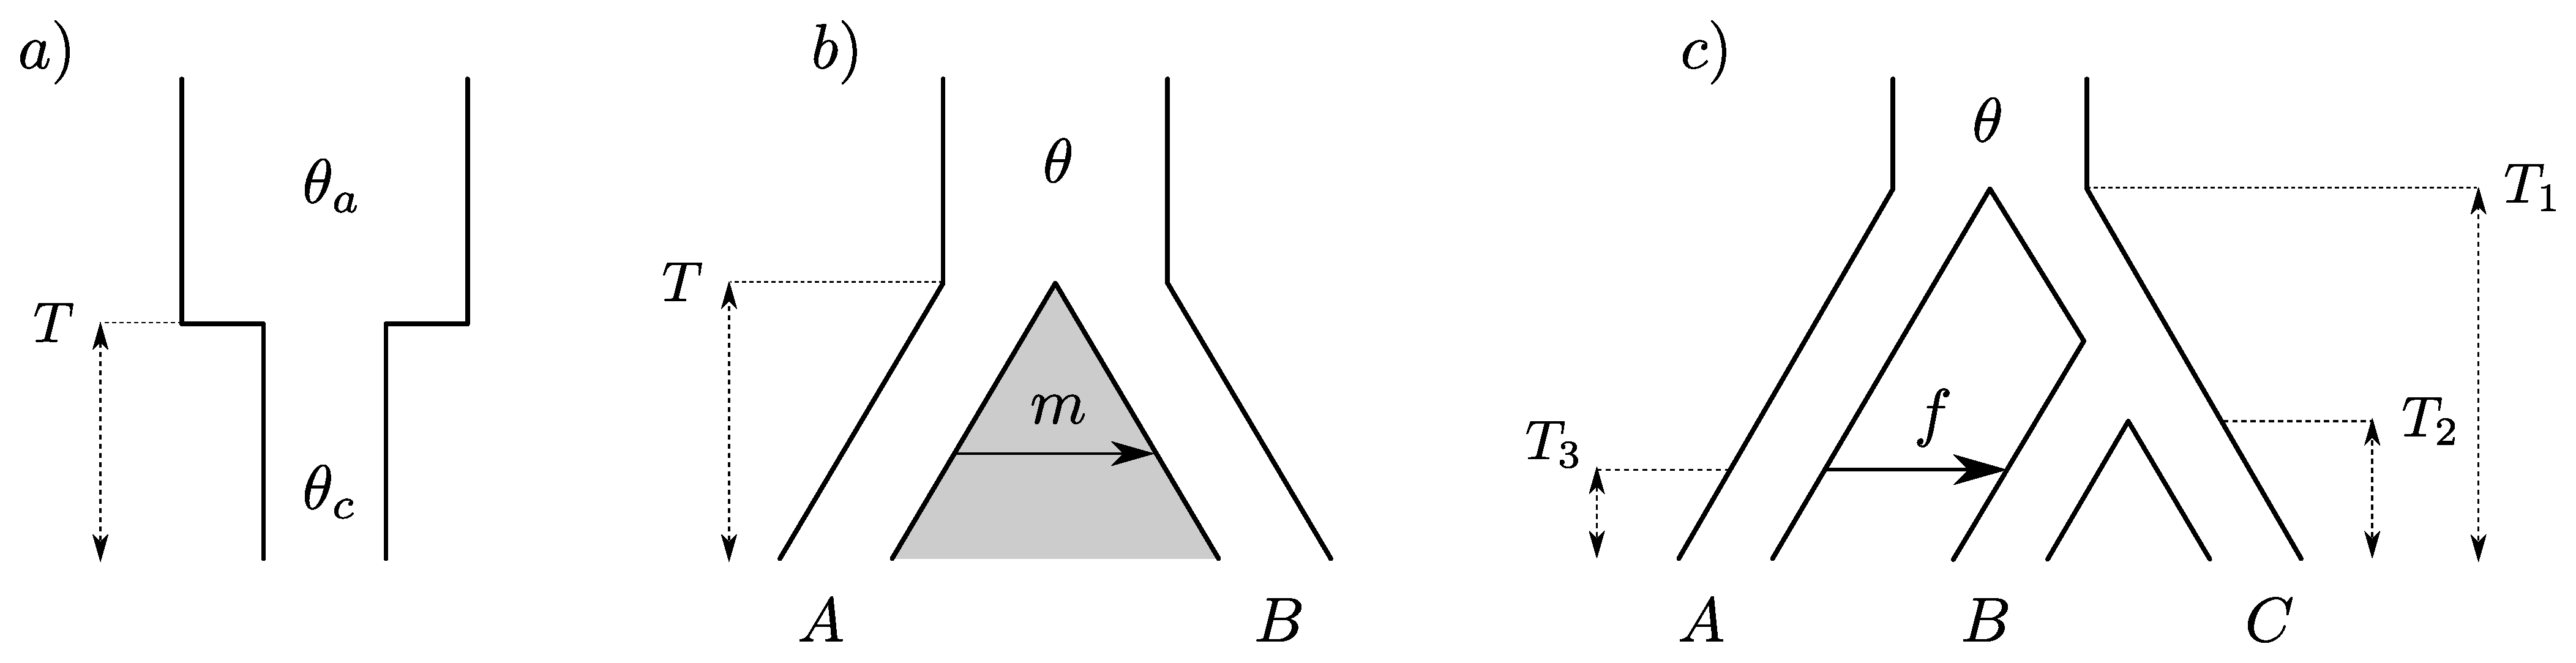
\includegraphics[width=1\textwidth]{models.pdf}
		
		\caption{Demographic models previously considered in the accompanying \href{http://dx.doi.org/10.1101/077958}{bioRxiv} draft. (\textit{a}) a single population with a sudden reduction in $N_e$, (\textit{b}) isolation between populations A and B followed by continuous unidirectional migration (from A to B) at rate $M$ migrants per generation and (\textit{c}) isolation between three populations A, B and C followed by unidirectional admixture of a fraction $f$ from A to B.}
		\label{fig:models}
	\end{tcolorbox}
\end{figure}


\subsubsection{The \textit{exact} bSFS}
\label{sec:examples_exact_bSFS}
\IndexSub{task}{exact\_bSFS}
Let us consider a single population sample of size 4 which doubled its effective population size at scaled time $ T = 0.2 $ in the past with $ \theta_{c} = 1 $ and $ \theta_{a} = 2 $ (\textit{see} Fig.~\ref{fig:models}a). We would like to calculate the exact \textit{folded} bSFS (\pref{key:task}) using 100K genealogies. The corresponding command line would look like 
\begin{codebox}
	\begin{verbatim}
	./ABLE 4 100000 -t 1 -eN 0.2 2 -T config_1pop_exact.txt
	\end{verbatim}
\end{codebox} 

along with the contents of \incode{config_1pop_exact.txt} as below
\begin{codebox}
	\begin{verbatim}
	pops 1 4

	kmax 4
	folded
	task exact_bSFS
	bSFS exact_bSFS.txt

	seed_PRNG 98368183
	\end{verbatim}
\end{codebox}

The \incode{kmax 4} (\pref{key:kmax}) is not a necessary option here and only serves to restrict the size of the bSFS by accounting explicitly for up to 3 SNPs per branch class in every block. A marginal probability class is calculated for all bSFS configurations having more then 3 SNPs per branch class. 


\subsubsection{The \textit{conditional} bSFS}
\label{sec:examples_conditional_bSFS}
\IndexSub{task}{conditional\_bSFS}
This example calculates the probabilities of observing only the bSFS configurations present in the data for a three population model. The parameter values used here are $ f_{A\rightarrow B} = 0.04 $, scaled population size $ \theta = 2.432 $, scaled times $ T_{3} = 0.0625 $, $ T_{2} = 0.075 $ and $ T_{1} = 0.3 $ (\textit{see} Fig.~\ref{fig:models}c).
\begin{codebox}
	\begin{lstlisting}[basicstyle=\ttfamily,breaklines=true,columns=fullflexible]
./ABLE 3 1000000 -t 2.432 -I 3 1 1 1 -es 0.0625 1 0.96 -ej 0.0625 4 3 -ej 0.075 1 2 -ej 0.3 2 3 -T config_3pop_conditional.txt
	\end{lstlisting}
\end{codebox}

And \incode{config_3pop_conditional.txt} contains :
\begin{codebox}
	\begin{verbatim}
	pops 3 1 1 1
	
	task conditional_bSFS
	datafile data_filename_to_be_specified_here.txt
	bSFS conditional_bSFS.txt
	
	seed_PRNG 12468192
	\end{verbatim}
\end{codebox}


\subsubsection{Inference with the bSFS}
\label{sec:examples_inference}
\IndexSub{task}{infer}
We now consider a two population example with 3 genomes in population A and 2 genomes in B (\textit{see} Fig.~\ref{fig:models}b) and blocks of size 500bp. This is a four parameter model with unidirectional gene flow at rate $ m $ after a split at time $ T $, with all scaled populations size parameters equal to $ \theta $ and scaled intra-block recombination rate $ \rho $. The parameters "\textit{to be inferred} $" : \theta $, $ \rho $, $ m $ and $ T $ have been respectively specified as \incode{tbi1}, \incode{tbi2}, \incode{tbi3} and \incode{tbi4} in the command line below. Note that the position corresponding to the number of genealogies to be sampled during inference (\incode{xxx} below) is entirely ignored by \ABLE\ and should only be specified in the config file.
\begin{codebox}
\begin{lstlisting}[basicstyle=\ttfamily,breaklines=true,columns=fullflexible]
./ABLE 5 xxx -t tbi1 -r tbi2 501 -I 2 3 2 -m 1 2 tbi3 -ej tbi4 1 2 -T config_2pop_infer.txt
\end{lstlisting}
\end{codebox}

The contents of \incode{config_2pop_infer.txt} below starts a global search immediately followed by a local search with the resulting MLE form the former.
\begin{codebox}
	\begin{verbatim}
	# general options
	# -----------------------
	pops 2 3 2
	task infer
	datafile data_filename_to_be_specified_here.txt
		seed_PRNG 29468147
	
	# global search options
	# -----------------------
	global_search CRS
	global_search_trees 50000
	global_search_evals 7000
	report_likelihoods 1000

	# parameter constraints
	# -----------------------
	global_upper_bound 15
	global_lower_bound 1e-2
	bounds tbi1 1e-2 1
	bounds tbi2 1e-2 1

	# local search options
	# -----------------------
	local_search_trees 50000
	refine_likelihoods 1000000
	\end{verbatim}
\end{codebox}

\printindex

\end{document}
